\documentclass{article}
\usepackage[T1]{fontenc}

% Language setting
\usepackage[french]{babel}

% Set page size and margins
\usepackage[a4paper,top=1cm,bottom=2cm,left=2cm,right=2cm]{geometry}

\usepackage{multicol}
\usepackage{tabularx}
\usepackage{longtable}
% Useful packages
\usepackage{amsmath}
\usepackage{graphicx}
\usepackage{float}
\usepackage{booktabs}
\usepackage{caption}
\usepackage{subcaption}
\usepackage{array}
\usepackage{hyperref}
\usepackage{url}
\usepackage{listings}
\usepackage{xcolor}
\usepackage{pgfplots}
\usepackage{fancyhdr}
\usepackage{lastpage} 

\pagestyle{fancy}
\fancyhf{} % On efface les entêtes et pieds de page par défaut

\renewcommand{\footrulewidth}{0.4pt}
\fancyfoot[L]{
\includegraphics[height=1cm]{images/logoCS.jpg}}
\fancyfoot[C]{\textit{Mention IA - Projet d'Apprentissage Automatique}}
\fancyfoot[R]{Page \thepage{} sur \pageref{LastPage}}

% Pour que le pied de page s'applique aussi sur la première page
\fancypagestyle{plain}{
    \fancyhf{} % Efface les entêtes et pieds de page par défaut de plain
    \fancyfoot[L]{
\includegraphics[height=1cm]{images/logoCS.jpg}}
    \fancyfoot[C]{\textit{Mention IA - Projet d'Apprentissage Automatique}}
    \fancyfoot[R]{Page \thepage{} sur \pageref{LastPage}}
    \renewcommand{\footrulewidth}{0.4pt} % Ligne horizontale
}

\pgfplotsset{compat=1.16}

\definecolor{codegray}{gray}{0.9}
\lstset{
    backgroundcolor=\color{codegray},
    basicstyle=\footnotesize\ttfamily,
    frame=single,
    breaklines=true,
    postbreak=\mbox{\textcolor{red}{$\hookrightarrow$}\space},
    showstringspaces=false,
    tabsize=4,
    captionpos=b
}

\title{Rapport de projet d'Apprentissage Automatique}
\author{
    \small Martin Rampont (martin.rampont@student-cs.fr) \and 
    \small Noémie Guisnel (noemie.guisnel@student-cs.fr) \and 
    \small Oscar Pastural (oscar.pastural@student-cs.fr) \and 
    \small Louis Gauthier (louis.gauthier@student-cs.fr) \and 
    \small Clément Florval (clement.florval@student-cs.fr)
}
\date{24 Octobre 2024 \\ Équipe 2}


\begin{document}
\maketitle
\tableofcontents
\newpage
\section{Problématique du projet}

Ce projet vise à développer un modèle de Machine Learning capable de prédire la qualité des soudures à partir de paramètres mécaniques, physiques et chimiques, obtenus sans recourir à des tests destructifs. L'objectif est d'identifier les facteurs influençant des propriétés clés comme la résistance à la traction, l'élasticité et la ductilité.

Dans des secteurs critiques tels que l'aéronautique et l'industrie pétrolière, la qualité des soudures est essentielle pour la sécurité et la fiabilité des infrastructures. Un modèle prédictif permettrait de prévenir les défauts de soudure, réduisant ainsi les risques d'accidents et les coûts liés aux réparations et tests destructifs.

\section{Analyse exploratoire des données et prétraitement}

\subsection{Exploration initiale des données et identification des variables cibles}

Le jeu de données comporte 1,652 observations et 46 variables, couvrant un large éventail d'informations sur les soudures. Ces variables incluent des concentrations d'éléments chimiques tels que le carbone, le manganèse et le nickel, des propriétés mécaniques comme la résistance à la traction, la limite d’élasticité et la dureté, ainsi que des caractéristiques microstructurales. Chaque observation représente un échantillon unique de soudure, identifiable par (\textit{Weld ID}).

L’objectif est de prédire la qualité des soudures en utilisant uniquement des variables mesurables avant la destruction de l'échantillon. En conséquence, les variables obtenues par des tests destructifs, comme la \textit{Yield strength}, l'\textit{Ultimate tensile strength} ou encore la \textit{Charpy impact toughness}, ne peuvent pas être incluses dans les variables d'entrée (features) de notre modèle. Ces variables seront plutôt utilisées comme variables cibles pour évaluer la qualité des soudures. La charpy temperature (température à laquelle le test Charpy est réalisé) n'est pas une variable à prédire, mais une variable d'entrée, car elle influe directement sur les résultats du test Charpy.

Le test Charpy, qui mesure la capacité d'un matériau à absorber de l'énergie avant de se casser, et les autres mesures mécaniques (résistance à la traction, élongation, etc.) ne sont généralement pas effectués simultanément sur le même échantillon, ce qui entraîne de nombreuses valeurs manquantes, classées comme MAR (Missing At Random). Nous avons initialement envisagé de séparer le dataset en deux pour prédire indépendamment les résultats du test Charpy et ceux des autres propriétés mécaniques. Cependant, cette approche a conduit à des résultats insatisfaisants pour le test Charpy en raison de la perte d'information. Nous avons donc opté pour conserver l'ensemble des données dans un même dataset pour améliorer la qualité des prédictions.\\

Ainsi, les variables cibles utilisables pour estimer la qualité des soudures incluent :

\begin{itemize} \item \textit{Yield strength / MPa} \item \textit{Ultimate tensile strength / MPa} \item \textit{Elongation / \%} \item \textit{Reduction of Area / \%} \item \textit{Charpy impact toughness / J} \end{itemize}

Nous avons également pris en compte la variable \textit{50 \% FATT} (température de transition fragile-ductile), mais elle présente un taux de valeurs manquantes de plus de 98 \%, la rendant inutilisable.

\subsection{Analyse des corrélations}

Afin de développer une intuition sur les relations entre les différentes variables du dataset, nous avons analysé les corrélations entre celles-ci. Pour ce faire, nous avons d’abord effectué quelques modifications sur les colonnes pour qu'elles soient exploitables :

\begin{longtable}{|p{4cm}|p{10cm}|}
\hline
\textbf{Catégorie} & \textbf{Changements Apportés} \\ \hline
\multicolumn{2}{|c|}{\textbf{Traitement des Colonnes Numériques}} \\ \hline
Colonnes avec signes $\leq$ & Les valeurs précédées du signe $\leq$ sont conservées telles quelles, sans modification, pour fournir une estimation utilisable tout en restant fidèle aux données originales. \\ \hline
\textit{Hardness / kg mm$^{-2}$} & Les annotations non pertinentes comme \textit{'158(Hv30)'} sont supprimées pour ne garder que la valeur numérique de la dureté. La colonne est ensuite convertie en valeurs numériques exploitables. \\ \hline
\textit{Interpass temperature / °C} & Les valeurs exprimées sous forme d’intervalles (\textit{150-200°C}) sont remplacées par la moyenne des bornes de l'intervalle afin de simplifier l'analyse. Les valeurs sont ensuite converties en données numériques. \\ \hline

\multicolumn{2}{|c|}{\textbf{Traitement des Colonnes Catégorielles}} \\ \hline
Encodage catégoriel & Un encodage \textit{one-hot} est réalisé pour les colonnes \textit{AC or DC} et \textit{Type of weld} afin de transformer les catégories en variables numériques. Une catégorie est supprimée dans chaque cas pour éviter la multicollinéarité. \\ \hline
\textit{Electrode positive or negative} & Les signes \textit{+} et \textit{-} sont transformés en valeurs numériques : \textit{1} pour une électrode positive et \textit{-1} pour une électrode négative, facilitant ainsi leur utilisation dans les modèles de machine learning. \\ \hline

\caption{Tableau récapitulatif des transformations de données correspondant au prétraitement effectué.}
\end{longtable}

Enfin, pour rendre toutes les colonnes exploitables dans notre modèle et permettre l'analyse des corrélations, nous avons transformé les colonnes de type object en valeurs numériques, soit sous forme d'entiers (int), soit de nombres flottants (float). Cela a permis de simplifier le traitement des données et d'assurer une compatibilité totale avec les outils d'analyse.\\

Une fois ce travail effectué, nous étudions les corrélations. 

Les corrélations les plus pertinentes pour notre étude concernent les variables liées directement à la qualité d'une soudure, telles que la \textit{résistance à la traction}, la \textit{limite d'élasticité}, l'\textit{élongation}, la \textit{résilience Charpy} et la \textit{réduction de section}. Voici quelques corrélations notables :

\begin{itemize} \item La \textbf{résistance à la traction} (\textit{Ultimate tensile strength}) est modérément corrélée à la concentration en chrome (0.48), suggérant que l'ajout de chrome améliore la résistance mécanique de la soudure. \item La \textbf{limite d'élasticité} (\textit{Yield strength}) montre une corrélation notable avec le tungstène (0.40), ce qui pourrait indiquer que cet élément influence la résistance aux déformations. \item L'\textbf{élongation} (\textit{Elongation}) présente une corrélation négative avec le chrome (-0.44), indiquant que des concentrations plus élevées de chrome peuvent diminuer la capacité d'allongement du matériau avant rupture. \item La \textbf{tenacité Charpy} (\textit{Charpy impact toughness}) est faiblement corrélée avec les concentrations chimiques, mais elle présente une forte corrélation avec la \textit{réduction de section} (0.83), ce qui est attendu, car une plus grande ductilité permet une meilleure absorption d'énergie avant la rupture. \end{itemize}

\subsection{Application d'une ACP}

\subsubsection{Gestion des outliers}

Nous avons identifié des valeurs aberrantes dans certaines variables. Par exemple, dans la variable \textit{Vanadium concentration / weight \%}, certaines valeurs dépassent largement les concentrations typiques. Au lieu de les supprimer, nous avons appliqué une winsorisation pour limiter l'impact de ces valeurs extrêmes tout en conservant leur information. Cette méthode permet de réduire l'influence des outliers tout en prenant en compte ces observations dans l'analyse.\\

\subsubsection{Gestion des valeurs manquantes}

Pour effectuer l'ACP et appliquer ensuite les modèles de Machine Learning, nous devons gérer les valeurs manquantes du dataset.
Nous supprimons les colonnes contenant trop de valeurs manquantes (plus de 80\%, considérées inexploitables et imputer des données risque de trop fausser les résultats). Cela supprime des colonnes comme \textit{Hardness} ou \textit{Primary Ferrite}.

D'autres variables présentent un taux de valeurs manquantes plus modéré, notamment des indicateurs clés de la qualité des soudures, tels que la \textit{Yield strength}, l'\textit{Ultimate tensile strength}, l'\textit{Elongation}, la \textit{Reduction of Area} et la \textit{Charpy impact toughness}. Comme vu dans l'analyse exploratoire des données, ces variables proviennent de tests destructifs ; par exemple, le test Charpy, qui mesure la \textit{Charpy impact toughness}, détruit la soudure, ce qui empêche de réaliser d'autres mesures comme la \textit{tensile strength} sur le même échantillon. De plus, nous avons remarqué que plusieurs tests étaient souvent réalisés sur des soudures identiques (ayant exactement les mêmes paramètres), avec un test de \textit{Yield strength} et \textit{UTS}, suivi de plusieurs tests Charpy à différentes températures. Pour traiter ces cas, nous avons regroupé les observations correspondant à une même soudure afin de combler les valeurs manquantes et d'éviter toute fuite de données (\textit{data leakage}) entre l'ensemble d'entraînement et les ensembles de test/validation.

Nous avons également comparé la distribution des cibles en fonction de la présence ou de l'absence de données pour chaque variable. Lorsque les distributions étaient similaires, nous avons considéré que les données manquaient de manière complètement aléatoire (MCAR) et avons imputé les valeurs manquantes avec la médiane. Pour les autres variables, où les données manquaient de manière conditionnelle (MAR), nous avons testé l'imputation par KNN, mais les meilleurs résultats ont été obtenus en imputant la médiane et en ajoutant une colonne binaire indiquant la présence ou non de données manquantes.

\subsubsection{Standardisation des Variables}

Avant d'appliquer l'ACP et les modèles de Machine Learning, nous avons standardisé les variables numériques à l'aide de la méthode de \textit{StandardScaler}, afin de leur donner une échelle comparable.

\subsubsection{Résultats de l'ACP}

Appliquer une ACP sur les variables numériques standardisées permet de réduire la dimensionnalité des données tout en préservant autant que possible la variance.

Nous avons examiné la variance expliquée cumulée en fonction du nombre de composantes principales. Nous avons choisi de conserver les 10 premières composantes, qui expliquent environ 80\,\% de la variance totale.

Nous avons visualisé les deux premières composantes principales en colorant les points en fonction de la variable cible \textit{Yield strength / MPa}. Cette visualisation permet de détecter des structures ou des regroupements dans les données.

\subsubsection{Clustering sur les résultats de l'ACP}
Nous avons appliqué un clustering par la méthode des k-means sur les résultats de l'ACP. Cette pratique est courante, le clustering devient alors plus efficace, car il opère sur des variables non corrélées, qui représentent les directions de plus grande variance dans les données. Cela aide à éviter les problèmes de multicolinéarité qui peuvent affecter les algorithmes de clustering. Nous avons également veillé à n'utiliser que les features en entrée afin de garantir que les groupes formés reflètent uniquement les structures présentes dans les données originales, sans influence des variables cibles.

Toutefois nous avons ensuite examiné la distribution des résultats de ce clustering par rapport à chaque variable cible (Figure~\ref{fig:inertia}). Cette analyse nous a permis de déterminer si les groupes obtenus se répercutent sur les outputs. Les résultats étaient modérés, mais nous avons observé des différences dans les distributions des variables cibles, en particulier pour le cluster 2, qui s'est distingué d'avantage.

De plus, nous avons utilisé l'ACP, en sélectionnant les cinq premières composantes principales lors de la méthode de représentation des features, pour vérifier l'impact des features sur les clusters générés. Cette analyse a confirmé l'importance relative des différentes concentrations mesurées dans le dataset. 

La méthode de l'inertie a été utilisée pour déterminer le nombre optimal de clusters. Pour rappel, l'inertie est définie par la formule suivante :

\[
I(k) = \sum_{i=1}^{k} \sum_{x_j \in C_i} \| x_j - \mu_i \|^2
\]

où \(I(k)\) est l'inertie pour \(k\) clusters, \(C_i\) est le \(i^{ème}\) cluster, \(x_j\) est un point de données dans \(C_i\), et \(\mu_i\) est le centroid du cluster \(C_i\).

\begin{figure}[H]
    \centering
    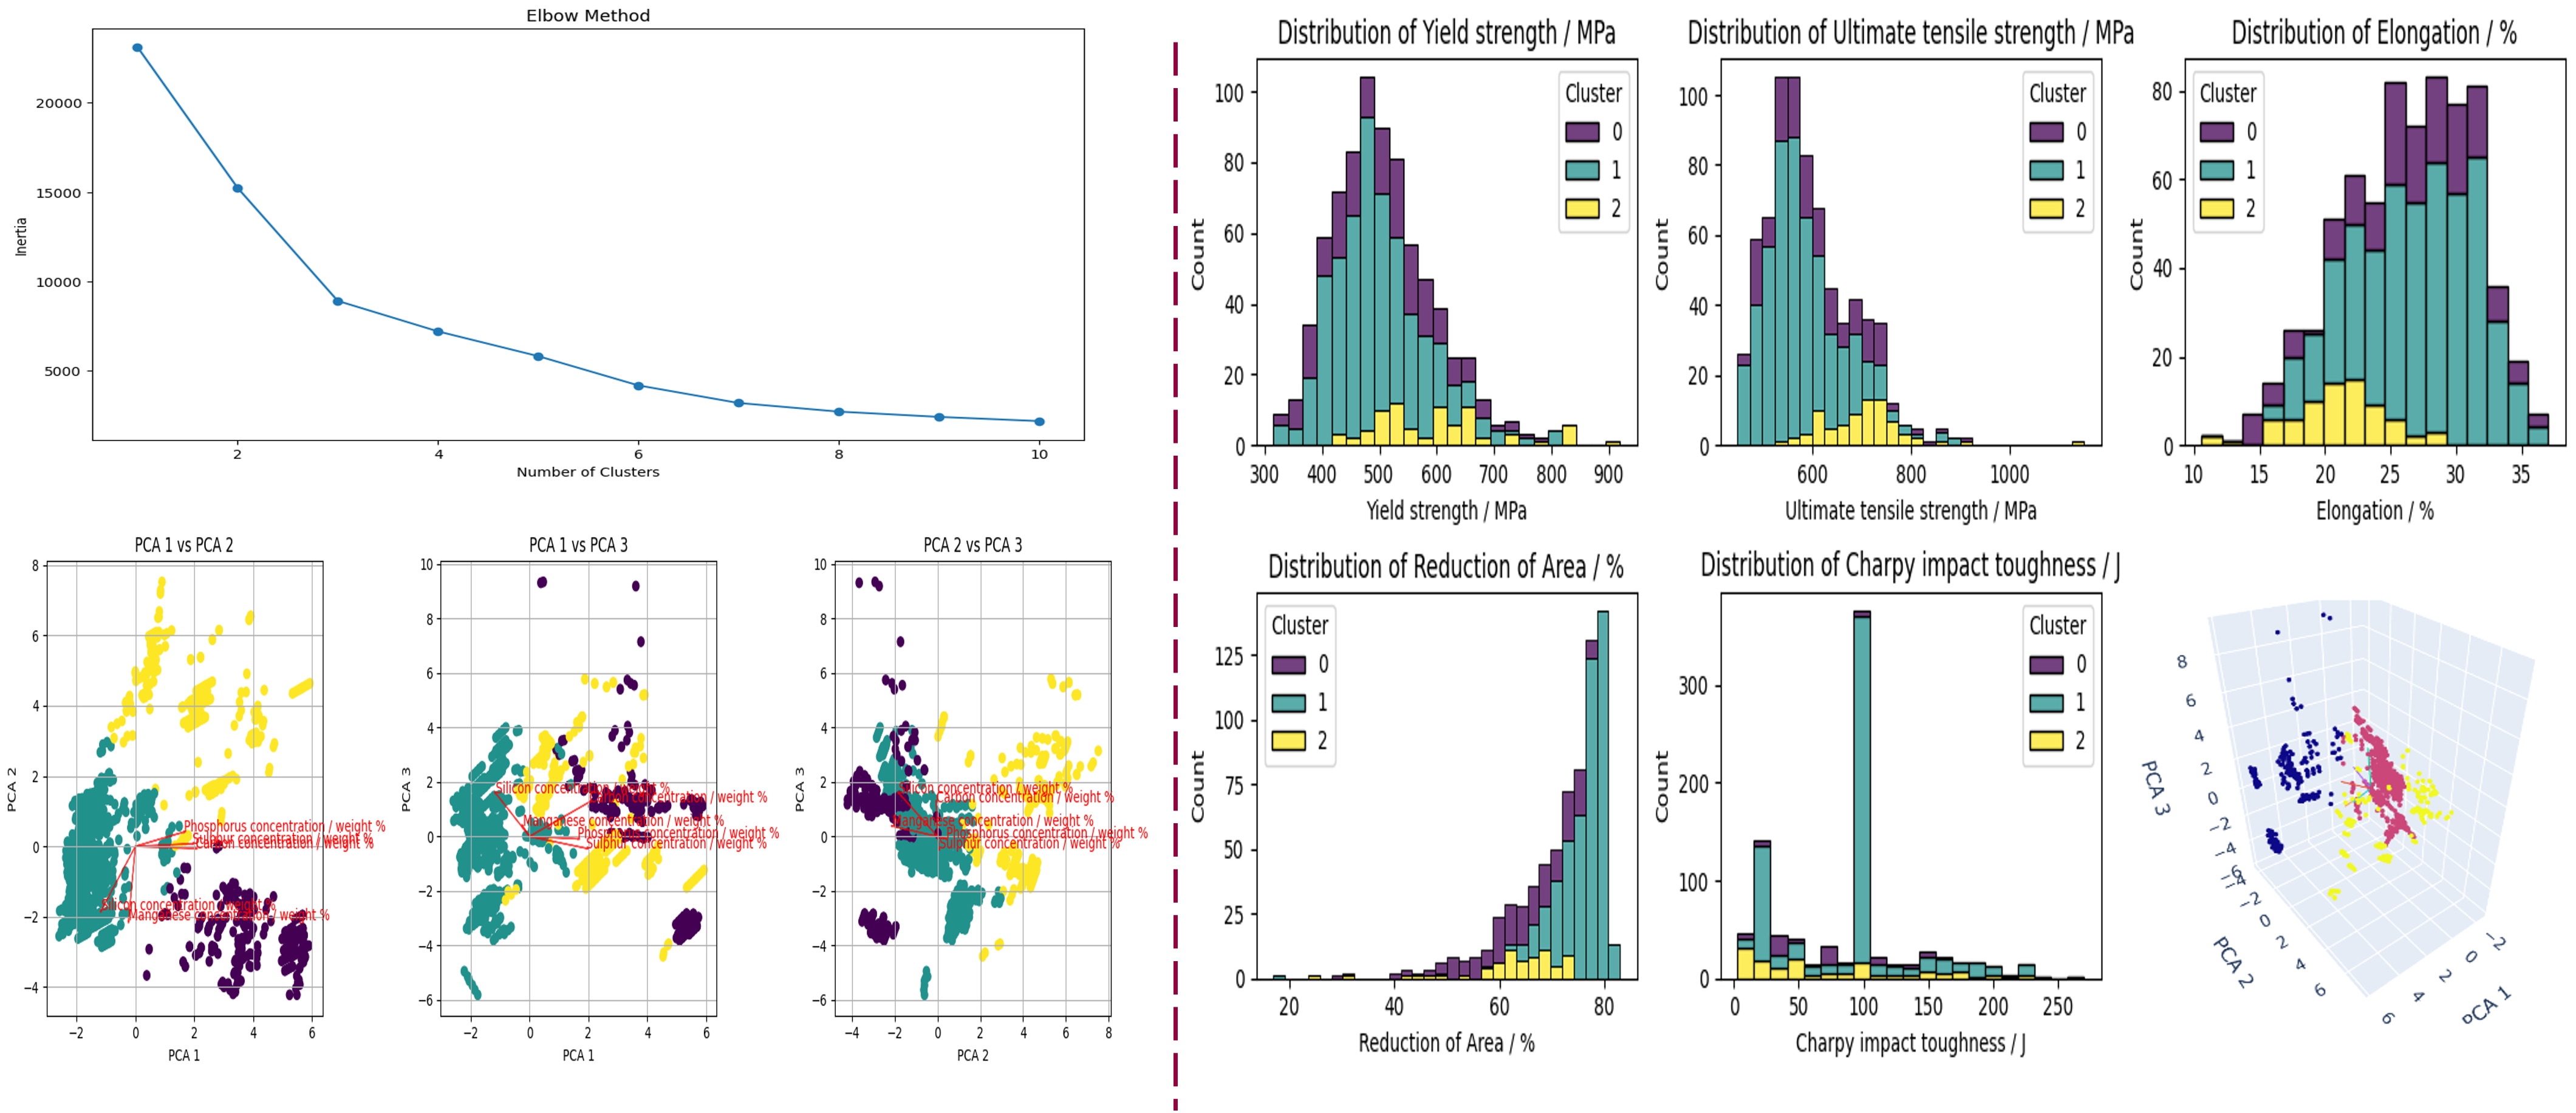
\includegraphics[width=\textwidth]{images/clustering.png}
    \caption{résultats du clustering k-means appliqué aux données de l'ACP, ainsi que les distributions des variables cibles par cluster}
    \label{fig:inertia}
\end{figure}

\section{Application des Algorithmes de Machine Learning}

\subsection{Sélection des Variables Cible}

Nous avons choisi de prédire plusieurs variables essentielles à la qualité des soudures : \textit{Yield strength / MPa}, \textit{Ultimate tensile strength / MPa}, \textit{Elongation / \%}, \textit{Reduction of Area / \%}, et \textit{Charpy impact toughness / J}. Ces variables sont des indicateurs clés qui permettent d’évaluer les propriétés mécaniques et la résistance globale des soudures, et donc leur qualité.

\subsection{Modèles Utilisés}

Durant notre phase de test, nous avons utilisé plusieurs modèles de régression :

\begin{itemize}
\item Régression Linéaire
\item Forêt d’arbres décisionnels (\textit{Random Forest})
\item Gradient Boosting
\item Machine à Vecteurs de Support (\textit{Support Vector Machine})
\item XGBoost
\end{itemize}

Après une phase d’expérimentation et d’optimisation des hyperparamètres via une recherche par grille (\textit{grid search}), nous avons retenu le modèle XGBoost. Celui-ci a montré des performances supérieures en termes de précision prédictive, tout en offrant une certaine explicabilité grâce à l’analyse de l’importance des caractéristiques (voir Figure~\ref{fig:xgboost_feature_importance}).

\begin{figure}[H]
    \centering
    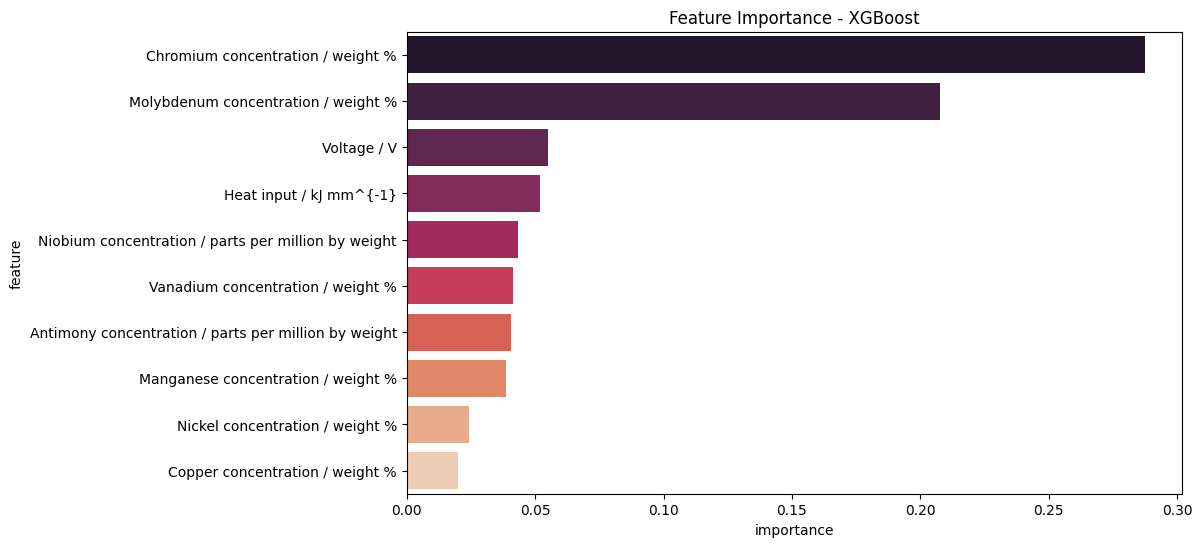
\includegraphics[width=0.7\textwidth]{images/xgboost_feature_importance.png}
    \caption{Importance des caractéristiques du modèle XGBoost}
    \label{fig:xgboost_feature_importance}
\end{figure}

Une partie exploratoire a été effectuée en parallèle, avec pour objectif de tester des prédictions multi-output en récupérant dynamiquement tous les modèles régressifs de scikit-learn. Cette exploration a permis de tester les modèles proposant nativement des prédictions multi-output ainsi que ceux compatibles avec l’implémentation \texttt{MultiOutputRegressor} de scikit-learn, qui permet de convertir un modèle single-output en modèle multi-output. Une cross-validation à 5 folds a été effectuée afin de mesurer la performance du modèle de régression tout en minimisant le risque de surajustement (overfitting). Cela a également permit de valider la généralisation des modèles. Des modèles externes usuels comme XGBoost ont également été intégrés à des fins de comparaison pour évaluer leurs performances dans un contexte multi-output. 

\subsection{Évaluation des Modèles}

Nous avons évalué nos modèles à l’aide de la validation croisée en utilisant la méthode \textit{GroupKFold}. Deux métriques de performance ont été retenues : l’erreur quadratique moyenne (RMSE) et le coefficient de détermination (R2). Le modèle XGBoost a montré les meilleures performances globales sur nos 5 variables cibles, avec une RMSE moyenne (standardisée) inférieure à 0,5 et un R2 élevé (>0.8), indiquant une bonne capacité de prédiction.

\subsection{Apprentissage semi-supervisé}

Initialement, nous avions envisagé l’utilisation d’une méthode d’apprentissage semi-supervisé basée sur l’auto-entraînement (\textit{self-training}) pour pallier les valeurs manquantes des variables cibles. Cependant, une analyse plus approfondie du jeu de données a révélé que la majorité des valeurs manquantes étaient en réalité dues à un mauvais regroupement des données dans le dataset, et non à des absences réelles de mesures. En conséquence, nous avons abandonné cette approche, d’autant plus que les tentatives d’utilisation de l’auto-entraînement n’ont pas donné de bons résultats.

\subsection{Résultats}

Le modèle final basé sur XGBoost a montré une précision élevée pour toutes les variables cibles sélectionnées, avec une bonne capacité de généralisation. La Figure~\ref{fig:predictions_vs_true} illustre la comparaison entre les valeurs prédites et les valeurs réelles pour la variable \textit{Yield strength / MPa}.

\begin{figure}[H]
    \centering
    \begin{subfigure}[b]{0.40\textwidth}
        \centering
        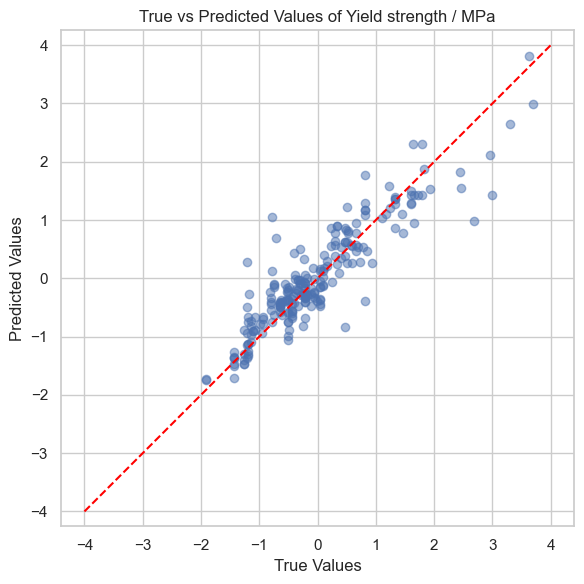
\includegraphics[width=\textwidth]{images/predictions_vs_true.png}
        % \caption{Comparaison entre les valeurs prédites et les valeurs réelles de \textit{Yield strength / MPa}}
        \label{fig:predictions_vs_true}
    \end{subfigure}
    \hfill
    \begin{subfigure}[b]{0.55\textwidth}
        \centering
        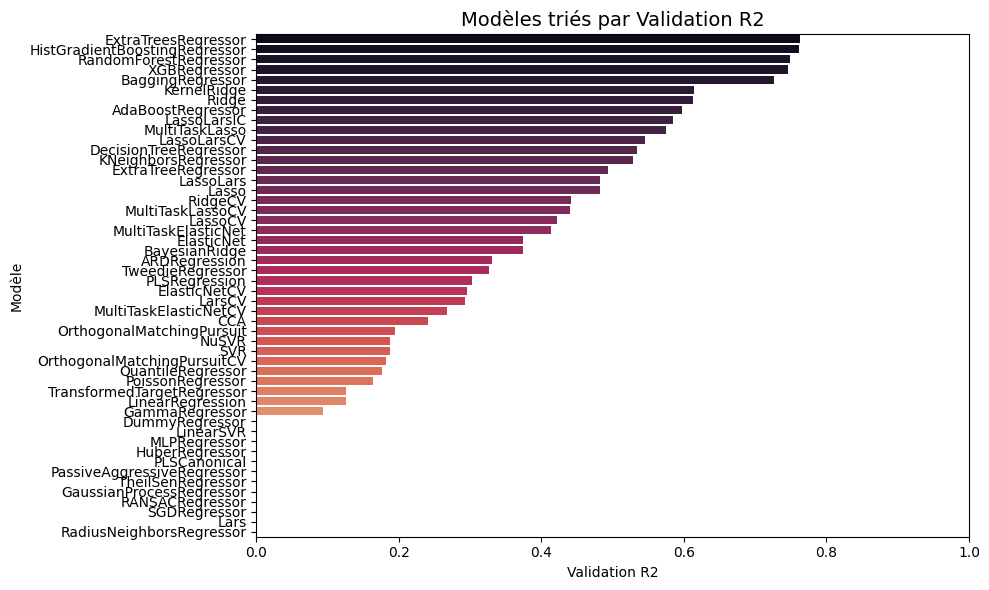
\includegraphics[width=\textwidth, height=0.25\textheight]{images/model_R2_results.png}
        % \caption{Résultats du score R2 des modèles (les scores R2 négatifs sont tronqués à 0)}
        \label{fig:second_image}
    \end{subfigure}
    \caption{(Gauche) Comparaison entre les valeurs prédites et les valeurs réelles de \textit{Yield strength / MPa}. (Droite) Classement des modèles en fonction de leur score R2 (validation), les scores R2 négatifs sont tronqués à 0.}
    \label{fig:side_by_side}
\end{figure}

\section{Développement d'une Interface Web}

Afin de rendre notre modèle accessible et de démontrer son utilité pratique, nous avons développé une application web à l'aide du framework Flask. Cette interface permet aux utilisateurs d'entrer manuellement les paramètres de soudure et d'obtenir une estimation de la qualité pour chaque variable cible ainsi qu'un score global.

De plus, l'application offre la possibilité d'uploader un fichier CSV contenant plusieurs échantillons de soudures. Le modèle prédit alors la qualité des soudures pour chaque échantillon, et un fichier CSV avec les prédictions peut être téléchargé.

Cette application web facilite l'interaction avec le modèle et permet une évaluation rapide de la qualité des soudures en fonction de différents paramètres. Elle pourrait être particulièrement utile pour les industriels souhaitant estimer la qualité de nouvelles soudures sans avoir à effectuer de tests destructifs immédiats.

\section{Conclusion}

Dans ce projet, nous avons démontré que les modèles ensemblistes, en particulier XGBoost, offrent des performances supérieures pour prédire la qualité des soudures à partir de paramètres mesurables sans tests destructifs. La spécificité du jeu de données, marqué par sa sparsité, certaines corrélations et des groupes de valeurs cibles, a nécessité une attention particulière. L’expertise métier a été au cœur du prétraitement, permettant de gérer efficacement ces particularités et de prêter une attention particulière à la gestion des variables cibles.

Pour rendre notre modèle accessible et opérationnel, nous avons mis à disposition une application web permettant la prédiction individuelle et le traitement par lots. Cette interface facilite l’intégration du modèle dans les processus industriels, offrant ainsi un outil pratique pour estimer rapidement la qualité des soudures.

En somme, ce travail illustre comment l’association de l’expertise métier et des techniques avancées d’apprentissage automatique peut aboutir à des solutions innovantes pour des problématiques industrielles complexes.

\newpage

\begin{thebibliography}{11}

\bibitem{olympus}
Olympus IMS, 
\textit{Détermination des défauts dans les soudures de tuyaux}, 
[En ligne]. Disponible : 
\url{https://www.olympus-ims.com/fr/applications/defect-sizing-pipe-welds/}

\bibitem{scikit-learn}
Scikit-learn, 
\textit{Machine Learning in Python}, 
[En ligne]. Disponible : 
\url{https://scikit-learn.org/stable/index.html}

\bibitem{pca}
Wikipedia, 
\textit{Analyse en Composantes Principales (PCA)}, 
[En ligne]. Disponible : 
\url{https://fr.wikipedia.org/wiki/Analyse_en_composantes_principales}

\bibitem{charpy}
ZwickRoell, 
\textit{Charpy Impact Test - Metals (ISO 148-1)}, 
[En ligne]. Disponible : 
\url{https://www.zwickroell.com/industries/materials-testing/impact-test/charpy-impact-test-metals-iso-148-1/#:~:text=This%20impact%20test%20is%20used%20to%20determine%20the...}

\bibitem{controle-visuel}
Contrôle Visuel, 
\textit{Normes de contrôle visuel des soudures}, 
[En ligne]. Disponible : 
\url{https://www.controle-visuel.com/normes-controle-visuel-soudure/}

\bibitem{eng-tips}
Eng-Tips, 
\textit{Thread : TOFD \& Weld Sizing}, 
[En ligne]. Disponible : 
\url{https://www.eng-tips.com/viewthread.cfm?qid=402830}

\bibitem{science-direct}
ScienceDirect, 
\textit{The Charpy Impact Test: Measuring Energy Absorbed}, 
[En ligne]. Disponible : 
\url{https://www.sciencedirect.com/topics/engineering/charpy-impact-test#:~:text=1.3.-,The%20Charpy%20impact%20test%20measures%20the%20energy%20absorbed...}

\bibitem{medium}
Hüseyin Coşgun, 
\textit{Dealing with Missing Data: From Zero to Advanced}, 
[En ligne]. Disponible : 
\url{https://medium.com/@hhuseyincosgun/dealing-with-missing-data-from-zero-to-advanced-4fb734ee5998}


\end{thebibliography}


\end{document}